
\begin{frame}
	\centering \LARGE \color{naranjaUCA} Introducción
\end{frame}
\begin{frame}{¿Qué es un proceso estocástico?}
	
\begin{itemize}
	\item Un \textbf{proceso estocástico }$\lbrace X_t, t \in T \rbrace$ es una colección de variables aleatorias definidas sobre el mismo espacio de probabilidad ($\Omega,S,P$). El conjunto $T$ se llama índice del proceso. Si $T$ es numerable diremos que el proceso estocástico es de tiempo discreto ($T=\lbrace 0,1,2,... \rbrace$) y si es continuo diremos que estamos ante un proceso estocástico de tiempo continuo ($T=\lbrace t, t\geq 0 \rbrace$).
	
\end{itemize}

\end{frame}
\begin{frame}{¿Qué es una cadena de Markov?}
	\begin{itemize}
		\item Sea $\lbrace X_n, n=0,1,2,...\rbrace$ un proceso estocástico de tiempo discreto. Suponemos que en cualquier instante, el proceso toma un número finito o numerable de valores (llamados estados del proceso).
		Un proceso estocástico de tiempo discreto es una \textbf{Cadena de Markov}, si para $t$=0,1,2,... y los estados $i_0, i_1,...,i_{n-1},i,j$:
		\pause
		$$
		P(X_{n+1}=j|X_n=i, X_{n-1}=i_{n-1},...,X_1=i_1, X_0=i_0)=
		$$ $$P(X_{n+1}=j|X_n=i_n)=p_{ij}
		$$
	\end{itemize}
\end{frame}

\begin{frame}{Ejemplo cadena de Markov}
	
	$$ 	\begin{array}{cccc}
	& 1 ~~ & 2 ~~ &  3
	\end{array}
	$$
	$$
	\begin{array}{c}
	1 \\ 2 \\ 3
	\end{array}
	\left(
	\begin{array}{ccc}
	1/3 & 1/3 & 1/3 \\
	1/3 & 0 & 2/3 \\
	1/2 & 1/2 & 0 \\
	\end{array}
	\right)
	$$
	
	\pause
	%\begin{figure*}[h]
		\centering
		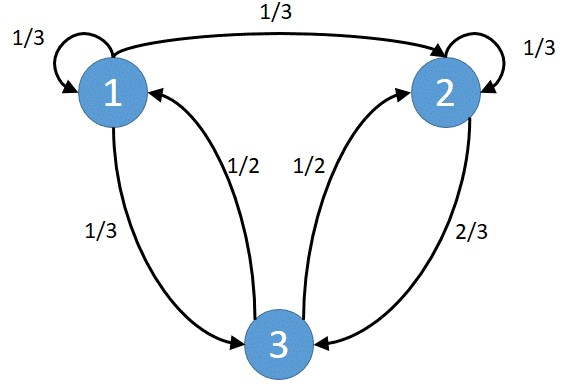
\includegraphics[width=0.4\textwidth]{grafo1}
		\label{grf1}
	%\end{figure*}
\end{frame}

\begin{frame}{¿Cuál es la probabilidad de estar en el estado $j$ después de n periodos?}
	$$
	p_{ij}^n=P(X_{m+n}=j|X_m)=P(X_n=j|X_0=i)
	$$
\end{frame}

\begin{frame}{Probabilidad de estado estable}
	Cuando $n$ es suficientemente grande
	$$
	p_{ij}^{n+1}\cong p_{ij}^n
	$$
	\pause
	En el límite
	$$
	lim ~  p_{ij}^n = \pi_j 
	$$
\end{frame}